\documentclass[english,serif,mathserif,xcolor=pdftex,dvipsnames,table]{beamer}
\usetheme{gc3}

\usepackage[T1]{fontenc}
\usepackage[utf8]{inputenc}
\usepackage{babel}

\usepackage{gc3}

\title[Sequencing tasks]{%
  Running tasks in parallel: \\
  \texttt{ParallelTaskCollection}
}
\author[R. Murri, S3IT UZH]{%
  Riccardo Murri \texttt{<riccardo.murri@uzh.ch>}
  \\[1ex]
  \emph{S3IT: Services and Support for Science IT}
  \\[1ex]
  University of Zurich
}
\date{January~23--27, 2017}


\begin{document}

% title frame
\maketitle


\begin{frame}[fragile]
  \frametitle{Basic use of ParallelTaskCollection}

\begin{python}
from gc3libs.workflow \
  import ParallelTaskCollection

class MyTasks~\HL{(ParallelTaskCollection)}~:
  # ...
  def __init__(self, ...):
    app1 = AnApp(...)
    app2 = AnotherApp(...)
    # ...
    appN = YetAnotherApp(...)
    ParallelTaskCollection.__init__(
      self, [app1, app2, ..., appN])
\end{python}

  \+ A \texttt{ParallelTaskCollection} runs a list of tasks, submitting
  at the same time as many as possible.
\end{frame}


\begin{frame}[fragile]
  \frametitle{Basic use of ParallelTaskCollection}

\begin{python}
from gc3libs.workflow \
  import ParallelTaskCollection

class MyTasks(ParalelTaskCollection):
  # ...
  def __init__(self, ...):
    app1 = AnApp(...)
    app2 = AnotherApp(...)
    # ...
    appN = YetAnotherApp(...)
    ParallelTaskCollection.__init__(
      self, ~\HL{[app1, app2, ..., appN]}~)
\end{python}

  \+
  Initialize a \texttt{ParallelTaskCollection} \\
  with a list of tasks to run.
\end{frame}


\begin{frame}[fragile]
  \frametitle{Running tasks in parallel}

\begin{python}
class MyScript(SessionBasedScript):
  # ...
  def new_tasks(self, extra):
    tasks_to_run = [
      MyTasks(...)
    ]
    return tasks_to_run
\end{python}

  \+ You can then run the entire collection by returning it from
  \lstinline|new_tasks()|, or by using it as a step in an outer
  \texttt{SequentialTaskCollection}.
\end{frame}


\begin{frame}[fragile]
  \frametitle{Detour: random colors}

  \href{http://www.imagemagick.org/script/color.php}{ImageMagick}
  allows specifying colors also by the syntax \texttt{xc:\#}$rgb$ where
  $r$, $g$, and $b$ are 2-digit hexadecimal numbers ranging from
  \texttt{00} to \texttt{ff}.

  \+
  For example, \texttt{\#ffa500} is the ``orange'' color.

  \+ You can generate these color specifications randomly from Python
  by combining \href{https://pyformat.info/}{string formatting} and the
  \href{https://docs.python.org/2/library/random.html#random.randint}{\texttt{randint}}
  function:
\begin{python}
  def random_color():
    from random import randint
    r = randint(0, 255)
    g = randint(0, 255)
    b = randint(0, 255)
    color = ("xc:#%02x%02x%02x" % (r, g, b))
    return color
\end{python}
\end{frame}


\begin{frame}
\begin{exercise*}[9.A]
  Write a \texttt{ParallelTaskCollection} class
  \texttt{RandomlyColorize} that is initialized with two parameters:
  an image file name \texttt{img} and a number \texttt{N}.

  \+
  The \texttt{RandomlyColorize} collection then consists of
  \texttt{N} instances of the \texttt{ColorizeApp}, each initialized
  with the same image file name \texttt{img} and three random colors.
\end{exercise*}
\end{frame}


\begin{frame}[fragile]
  \frametitle{Detour: image montage}

\begin{sh}
$ montage \
    cyan.jpg magenta.jpg yellow.jpg black.jpg \
    -tile 2x2 -geometry +0+0 cmyk.jpg
\end{sh}%$

  \+
  \begin{tabular}[c]{ccc}
    \begin{minipage}[c]{0.45\linewidth}
      
\includegraphics[width=0.2\textwidth]{fig/cyan.jpg}    \textbf{,}
      
\includegraphics[width=0.2\textwidth]{fig/magenta.jpg} \textbf{,}
      
\includegraphics[width=0.2\textwidth]{fig/yellow.jpg}  \textbf{,}
      \includegraphics[width=0.2\textwidth]{fig/black.jpg}
      \vspace{0.2\textheight}
    \end{minipage}
    &
    {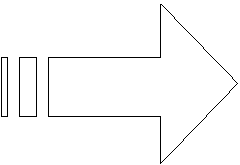
\includegraphics[width=0.1\linewidth,totalheight=0.25\textheight]{fig/arrow.pdf}}
    &
    
\includegraphics[width=0.2\textwidth]{fig/cmyk.jpg}
  \end{tabular}
\end{frame}


\begin{frame}
  {\small Write your own ``Warholize'' workflow!}

  \small

  \+
  \begin{exercise*}[9.B]
    Write a \texttt{WarholizeScript} session-based script.

    \+
    The script takes any number of image file names as arguments;
    each image undergoes the following processing steps:
    \begin{enumerate}
    \item Conversion to grayscale;
    \item From the grayscaled version, $N^2$ randomly-colored new images are formed;
    \item These $N^2$ tiles are arranged in a $N \times N$ grid, which
      is the final result of the processing pipeline.
    \end{enumerate}

    \+
    A command-line option \texttt{-{}-size} allows one to set the
    value of $N$, with default $N=2$.
  \end{exercise*}
\end{frame}


\end{document}

%%% Local Variables:
%%% mode: latex
%%% TeX-master: t
%%% End:
